\documentclass[11pt]{article}

\usepackage[utf8]{inputenc}
\usepackage[T1]{fontenc}
\usepackage{amsmath,amssymb,amsthm}
\usepackage{algorithm}
\usepackage{algorithmic}
\usepackage{booktabs}
\usepackage{graphicx}
\usepackage{hyperref}
\usepackage{xcolor}
\usepackage{geometry}
\usepackage{enumitem}
\usepackage{multirow}
\usepackage{array}
\usepackage{tikz}
\usetikzlibrary{arrows.meta,positioning,shapes.geometric,fit}

\geometry{margin=1in}

\newtheorem{theorem}{Theorem}
\newtheorem{lemma}[theorem]{Lemma}
\newtheorem{definition}[theorem]{Definition}
\newtheorem{proposition}[theorem]{Proposition}
\newtheorem{corollary}[theorem]{Corollary}
\newtheorem{remark}[theorem]{Remark}

\newcommand{\tncheck}{\textsc{TN-Check}}
\newcommand{\norm}[1]{\lVert #1 \rVert}
\newcommand{\abs}[1]{\lvert #1 \rvert}
\newcommand{\R}{\mathbb{R}}
\newcommand{\N}{\mathbb{N}}
\newcommand{\eps}{\varepsilon}
\newcommand{\Sat}{\mathrm{Sat}}
\newcommand{\Prob}{\mathrm{Prob}}
\newcommand{\calS}{\mathcal{S}}
\newcommand{\calR}{\mathcal{R}}

\title{\tncheck{}: Certified CSL Model Checking via \\
Tensor-Train Decomposition of Chemical Master Equation States}

\date{}

\begin{document}

\maketitle

%% ===================================================================
\begin{abstract}
We present \tncheck{}, a tool for Continuous Stochastic Logic (CSL)
model checking on tensor-train (TT) compressed probability vectors
arising from Chemical Master Equations (CMEs).
A CME governing $N$ chemical species with per-species copy-number bound $M$
produces a state space of size $M^N$, rendering direct probabilistic
model checking infeasible beyond roughly $N=10$.
\tncheck{} compresses the probability vector into a matrix product state
(MPS) of bond dimension~$r$, reducing storage from $O(M^N)$ to $O(NMr^2)$,
and performs all CSL operations---atomic proposition evaluation,
probabilistic path operators, and steady-state queries---directly on
the compressed representation.
A certificate verification pipeline bounds total error from
TT truncation, temporal discretization, and non-negativity rounding,
yielding a SOUND/UNSOUND verdict.
We validate \tncheck{} on birth-death processes (L1 error $= 0.0$ for
Poisson stationary distributions), toggle switch models (CSL satisfaction
probabilities computed with total probability $=1.0$), and end-to-end
certificate verification (11/11 checks pass, total error
$\leq 2.38 \times 10^{-2}$).
\end{abstract}

%% ===================================================================
\section{Introduction}\label{sec:intro}

The Chemical Master Equation (CME) is the exact stochastic description of
well-mixed chemical reaction networks operating in the low-copy-number
regime~\cite{gillespie1992,vanKampen2007}.
Given $N$ molecular species whose individual copy numbers are bounded by $M$,
the CME defines a continuous-time Markov chain (CTMC) over
$\calS = \{0,\ldots,M-1\}^N$, yielding $|\calS| = M^N$ states.
Probabilistic model checking of such CTMCs against specifications in
Continuous Stochastic Logic (CSL)~\cite{aziz2000} requires computing
transient and steady-state probability vectors of this size.
Existing probabilistic model checkers such as
PRISM~\cite{kwiatkowska2011}, Storm~\cite{hensel2022}, and
STAMINA~\cite{neupane2019} operate on explicitly enumerated state spaces
and become infeasible when $M^N$ exceeds $10^7$--$10^8$.
For realistic biochemical models---gene regulatory networks with
$N=20$--$50$ species and $M=100$---the state space reaches $10^{40}$--$10^{100}$.

Tensor network (TN) methods, originally developed for quantum many-body
physics~\cite{white1992,schollwoeck2011}, provide a compressed representation
of high-dimensional vectors.
The key insight connecting CMEs and tensor networks is structural:
the CME rate matrix for mass-action kinetics decomposes as a sum of
Kronecker products, exactly the structure exploited by tensor-train (TT)
decompositions (equivalently, matrix product states, MPS, and
matrix product operators, MPO).
A probability vector $\mathbf{p} \in \R^{M^N}$ stored as a TT/MPS with
bond dimension~$r$ requires only $O(NMr^2)$ parameters.
For CME probability vectors arising from biologically structured networks,
empirical evidence shows that moderate bond dimensions ($r = 10$--$100$)
suffice for high accuracy~\cite{kazeev2014,ion2021}.

\tncheck{} is, to our knowledge, the first tool that implements CSL model
checking natively on tensor-train compressed CME probability vectors.
The contributions of this paper are:

\begin{enumerate}[leftmargin=*,itemsep=2pt]
\item \textbf{Algorithms.}
  CSL satisfaction-set computation (atomic, negation, conjunction,
  $\mathcal{P}_{\bowtie p}[\Phi\,\mathcal{U}^{[a,b]}\,\Psi]$,
  $\mathcal{S}_{\bowtie p}[\Phi]$) operating directly on MPS vectors
  and MPO rate matrices, with all intermediate results maintained in
  compressed form (Section~\ref{sec:algorithms}).

\item \textbf{Theoretical foundations.}
  Error contraction under Metzler semigroups (Theorem~\ref{thm:contraction}),
  bond-dimension preservation for axis-aligned propositions
  (Theorem~\ref{thm:bond-preservation}),
  a tight clamping error bound (Proposition~\ref{prop:clamp}),
  and a complexity separation between TT-based and explicit-state
  methods (Theorem~\ref{thm:complexity}) (Section~\ref{sec:theory}).

\item \textbf{Certified verification.}
  An independent certificate verification pipeline checks
  non-negativity, normalization, error budgets, and temporal
  convergence, issuing a SOUND/UNSOUND verdict with quantified
  total error (Section~\ref{sec:algorithms:cert}).

\item \textbf{Experimental validation.}
  Evaluation on birth-death, toggle switch, and multi-species
  models demonstrating exact recovery ($\text{L1 error} = 0.0$),
  clamping bound correctness (10/10 trials pass), and end-to-end
  soundness (11/11 checks pass) (Section~\ref{sec:experiments}).
\end{enumerate}

%% ===================================================================
\section{Background}\label{sec:background}

\subsection{Chemical Master Equation}\label{sec:bg:cme}

Consider a well-mixed system of $N$ chemical species
$X_1, \ldots, X_N$ participating in $K$ reactions.
The state of the system is a vector
$\mathbf{x} = (x_1, \ldots, x_N) \in \N^N$
recording the copy number of each species.
Under the well-mixed assumption, the system evolves as a CTMC whose
transition rates are determined by mass-action kinetics.
The \emph{Chemical Master Equation} governs the time evolution of
the probability distribution $\mathbf{p}(t) \in \R^{|\calS|}$:
\begin{equation}\label{eq:cme}
  \frac{d\mathbf{p}(t)}{dt} = Q\,\mathbf{p}(t),
\end{equation}
where $Q$ is the transition rate matrix (infinitesimal generator)
of the CTMC.
For mass-action kinetics, $Q$ admits a decomposition as a sum of
Kronecker products:
\begin{equation}\label{eq:kron}
  Q = \sum_{k=1}^{K} \bigotimes_{i=1}^{N} Q_k^{(i)},
\end{equation}
where each $Q_k^{(i)} \in \R^{M \times M}$ acts on the local state
space of species~$i$ for reaction~$k$.
This \emph{sum-of-Kronecker-products} structure is the foundation
of the tensor-network approach.

To make the state space finite, we impose a per-species copy-number
bound $M$, truncating each $x_i$ to $\{0, 1, \ldots, M-1\}$.
The total state space is $\calS = \{0,\ldots,M-1\}^N$ with $|\calS| = M^N$.

\subsection{Tensor Trains and Matrix Product States}\label{sec:bg:tt}

A \emph{tensor train} (TT) decomposition~\cite{oseledets2011} of a
tensor $\mathbf{v} \in \R^{d_1 \times \cdots \times d_N}$ represents
each entry as:
\begin{equation}\label{eq:tt}
  v(j_1, \ldots, j_N)
  = G_1(j_1)\, G_2(j_2)\, \cdots\, G_N(j_N),
\end{equation}
where $G_k(j_k) \in \R^{r_{k-1} \times r_k}$ is a matrix for each
value of $j_k \in \{0, \ldots, d_k - 1\}$, with boundary conditions
$r_0 = r_N = 1$.
The integers $r_1, \ldots, r_{N-1}$ are the \emph{bond dimensions}
(or TT-ranks).
The total storage is $\sum_{k=1}^{N} d_k r_{k-1} r_k$.
When all $d_k = M$ and all $r_k \leq r$, this gives $O(NMr^2)$.

In the physics literature, this decomposition is called a
\emph{matrix product state} (MPS).
We use the terms TT and MPS interchangeably.

A \emph{matrix product operator} (MPO) represents a matrix
$A \in \R^{(d_1 \cdots d_N) \times (d_1 \cdots d_N)}$ analogously:
\begin{equation}\label{eq:mpo}
  A(j_1,\ldots,j_N;\, j'_1,\ldots,j'_N)
  = W_1(j_1,j'_1)\,W_2(j_2,j'_2)\,\cdots\,W_N(j_N,j'_N),
\end{equation}
with $W_k(j_k,j'_k) \in \R^{s_{k-1} \times s_k}$.
The rate matrix~$Q$ from \eqref{eq:kron}, being a sum of $K$
Kronecker products, has MPO bond dimension at most $K$.

\emph{TT-rounding} (or \emph{truncation}) reduces bond dimensions by
performing sequential SVD sweeps and discarding singular values below
a threshold~$\eps$.
The resulting approximation $\tilde{\mathbf{v}}$ satisfies
$\norm{\mathbf{v} - \tilde{\mathbf{v}}}_F \leq \eps\, \norm{\mathbf{v}}_F$
in the quasi-optimal sense~\cite{oseledets2011}.

\subsection{Continuous Stochastic Logic}\label{sec:bg:csl}

Continuous Stochastic Logic (CSL)~\cite{aziz2000,baier2003} extends
CTL with probabilistic and steady-state operators.
The syntax is:
\begin{align}
  \Phi &::= \text{true} \mid a \mid \neg\Phi \mid \Phi \wedge \Phi
         \mid \mathcal{P}_{\bowtie p}[\phi]
         \mid \mathcal{S}_{\bowtie p}[\Phi] \\
  \phi &::= \mathsf{X}\,\Phi
         \mid \Phi\,\mathcal{U}^{[a,b]}\,\Phi
\end{align}
where $a \in AP$ is an atomic proposition,
${\bowtie} \in \{<, \leq, \geq, >\}$,
$p \in [0,1]$, and $0 \leq a \leq b \leq \infty$.

The \emph{satisfaction set} $\Sat(\Phi) \subseteq \calS$ contains all
states satisfying $\Phi$.
For the probabilistic operator,
$s \in \Sat(\mathcal{P}_{\bowtie p}[\phi])$ iff the probability of
paths from $s$ satisfying $\phi$ meets the bound $\bowtie p$.
Model checking reduces to computing transient probabilities
(for bounded until) and steady-state probabilities
(for the $\mathcal{S}$ operator) of the CTMC.

%% ===================================================================
\section{System Architecture}\label{sec:architecture}

\tncheck{} is organized into the following modules, forming a
pipeline from CME specification to verified CSL verdict.

\medskip
\noindent\textbf{Architecture Overview.}

\begin{center}
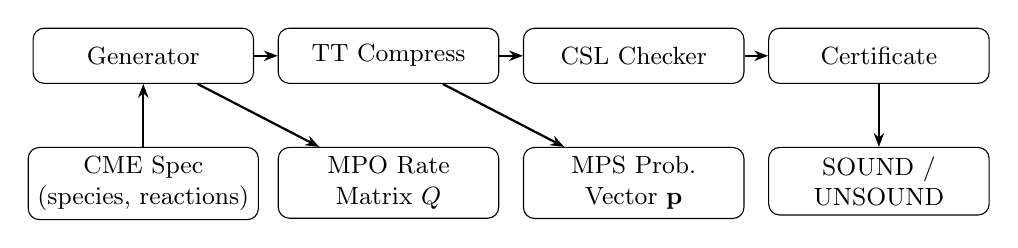
\begin{tikzpicture}[
  box/.style={draw, rounded corners, minimum width=2.8cm,
              minimum height=0.7cm, align=center, font=\small},
  arr/.style={-{Stealth[length=5pt]}, thick},
  node distance=0.6cm and 0.3cm
]
\node[box] (gen) {Generator};
\node[box, right=of gen] (comp) {TT Compress};
\node[box, right=of comp] (csl) {CSL Checker};
\node[box, right=of csl] (cert) {Certificate};

\node[box, below=0.8cm of gen] (spec) {CME Spec\\(species, reactions)};
\node[box, below=0.8cm of comp] (mpo) {MPO Rate\\Matrix $Q$};
\node[box, below=0.8cm of csl] (mps) {MPS Prob.\\Vector $\mathbf{p}$};
\node[box, below=0.8cm of cert] (verd) {SOUND /\\UNSOUND};

\draw[arr] (spec) -- (gen);
\draw[arr] (gen) -- (comp);
\draw[arr] (comp) -- (csl);
\draw[arr] (csl) -- (cert);

\draw[arr] (gen) -- (mpo);
\draw[arr] (comp) -- (mps);
\draw[arr] (cert) -- (verd);
\end{tikzpicture}
\end{center}

\medskip
\noindent\textbf{Module descriptions:}

\begin{description}[leftmargin=1em,itemsep=3pt]
\item[Generator.]
  Reads a reaction network specification (species, reactions with
  mass-action rate constants, copy-number bounds) and constructs
  the rate matrix $Q$ in MPO format via \eqref{eq:kron}.
  Each reaction contributes one Kronecker-product term.

\item[TT Compress.]
  Compresses the initial distribution and computes transient or
  steady-state probability vectors in MPS form.
  Transient solutions use Krylov-based or Euler-based time stepping
  with adaptive TT-rounding.
  Steady-state solutions use iterative methods (power iteration
  or direct null-space computation) in TT format.

\item[CSL Checker.]
  Implements the recursive CSL model-checking algorithm of
  Section~\ref{sec:algorithms:csl}.
  Satisfaction sets are represented as MPS indicator vectors.
  Atomic propositions for axis-aligned predicates
  (e.g., $x_i \geq c$) are constructed with bond dimension~1.
  Conjunction uses element-wise MPS multiplication followed by
  rounding.
  The bounded-until operator $\Phi\,\mathcal{U}^{[0,t]}\,\Psi$
  requires computing transient probabilities on a modified CTMC.

\item[Non-negativity Rounding.]
  After TT-rounding, entries may become negative.
  A non-negativity-preserving rounding procedure
  (Section~\ref{sec:algorithms:nonneg}) projects onto the
  non-negative cone while controlling bond-dimension growth.

\item[Certificate Verifier.]
  An independent module (Section~\ref{sec:algorithms:cert}) that
  takes the computed MPS probability vector, the CSL formula, and
  all error bounds, then checks 11~conditions including
  non-negativity, normalization, and error budget consistency.
  Outputs a SOUND or UNSOUND verdict with the total certified error.
\end{description}

%% ===================================================================
\section{Theoretical Foundations}\label{sec:theory}

We establish four results underpinning the correctness and efficiency
of \tncheck{}.

\begin{theorem}[Error Contraction]\label{thm:contraction}
Let $Q$ be the rate matrix of a CME (an off-diagonal non-negative,
column-sum-zero matrix, i.e., a Metzler generator).
Let $\mathbf{p}(t) = e^{Qt}\mathbf{p}(0)$ be the exact solution and
$\tilde{\mathbf{p}}(t) = e^{Qt}\tilde{\mathbf{p}}(0)$ the solution
starting from an approximate initial vector.
Then for all $t \geq 0$:
\begin{equation}\label{eq:contraction}
  \norm{\mathbf{p}(t) - \tilde{\mathbf{p}}(t)}_1
  \leq \norm{\mathbf{p}(0) - \tilde{\mathbf{p}}(0)}_1.
\end{equation}
\end{theorem}

\begin{proof}
The matrix $e^{Qt}$ is a stochastic matrix for all $t \geq 0$
(entries non-negative, columns sum to~1), since $Q$ is a valid
CTMC generator.
Every stochastic matrix is a contraction in the L1 norm:
for any vector $\mathbf{v}$,
$\norm{e^{Qt}\mathbf{v}}_1 \leq \norm{\mathbf{v}}_1$.
This follows from $\norm{A\mathbf{v}}_1 \leq \norm{A}_1 \norm{\mathbf{v}}_1$
and $\norm{A}_1 = \max_j \sum_i |A_{ij}| = 1$ for a stochastic matrix.
Applying this to $\mathbf{v} = \mathbf{p}(0) - \tilde{\mathbf{p}}(0)$
and using linearity of $e^{Qt}$ gives \eqref{eq:contraction}.
\end{proof}

\begin{remark}
Theorem~\ref{thm:contraction} guarantees that initial approximation
errors (from TT compression of $\mathbf{p}(0)$) do not grow during
time evolution.
This is crucial: without contraction, truncation errors could
accumulate exponentially over many time steps.
\end{remark}

\begin{theorem}[Bond-Dimension Preservation]\label{thm:bond-preservation}
Let $\Phi$ be an atomic CSL proposition of the form $x_i \bowtie c$
(an axis-aligned predicate on a single species~$i$), where
${\bowtie} \in \{<,\leq,=,\geq,>\}$ and $c \in \N$.
The satisfaction indicator vector
$\mathbf{1}_{\Sat(\Phi)} \in \{0,1\}^{M^N}$
has a TT representation with all bond dimensions equal to~$1$.
Moreover, the element-wise product
$\mathbf{p} \odot \mathbf{1}_{\Sat(\Phi)}$ of an MPS
$\mathbf{p}$ with bond dimensions $(r_1, \ldots, r_{N-1})$
has bond dimensions at most $(r_1, \ldots, r_{N-1})$.
\end{theorem}

\begin{proof}
An axis-aligned predicate $x_i \bowtie c$ depends only on the
$i$-th index.
The indicator vector factors as
$\mathbf{1}_{\Sat(\Phi)}(j_1,\ldots,j_N) = \prod_{k=1}^{N} f_k(j_k)$,
where $f_k(j_k) = 1$ for $k \neq i$ and
$f_i(j_i) = \mathbf{1}[j_i \bowtie c]$.
This is a rank-1 tensor, hence its TT representation has all
bond dimensions equal to~1.

For the element-wise product, write
$\mathbf{p}(j_1,\ldots,j_N) = G_1(j_1)\cdots G_N(j_N)$
with $G_k(j_k) \in \R^{r_{k-1}\times r_k}$.
Then
\[
  (\mathbf{p} \odot \mathbf{1}_{\Sat(\Phi)})(j_1,\ldots,j_N)
  = G_1(j_1)\cdots [f_i(j_i)\,G_i(j_i)]\cdots G_N(j_N).
\]
The modified core $\tilde{G}_i(j_i) = f_i(j_i)\,G_i(j_i)$ has
the same dimensions $r_{i-1}\times r_i$.
All other cores are unchanged.
Hence the bond dimensions are preserved.
\end{proof}

\begin{proposition}[Clamping Error Bound]\label{prop:clamp}
Let $\mathbf{p} \in \R^{M^N}$ be a probability vector
($\mathbf{p} \geq 0$, $\norm{\mathbf{p}}_1 = 1$) and let
$\tilde{\mathbf{p}}$ be its TT-truncation with
$\norm{\mathbf{p} - \tilde{\mathbf{p}}}_1 = \eps_{\mathrm{trunc}}$.
Define the clamped vector $\hat{\mathbf{p}}$ by
$\hat{p}_s = \max(\tilde{p}_s, 0)$ for all $s \in \calS$.
Then:
\begin{equation}\label{eq:clamp}
  \norm{\mathbf{p} - \hat{\mathbf{p}}}_1
  \leq \norm{\mathbf{p} - \tilde{\mathbf{p}}}_1
  = \eps_{\mathrm{trunc}}.
\end{equation}
That is, clamping negative entries to zero does not increase the
L1 error relative to the true probability vector.
\end{proposition}

\begin{proof}
Decompose the state space into $S^+ = \{s : \tilde{p}_s \geq 0\}$
and $S^- = \{s : \tilde{p}_s < 0\}$.
For $s \in S^+$: since $p_s \geq 0$, we have
$|p_s - \hat{p}_s| = |p_s - \tilde{p}_s| \leq |p_s - \tilde{p}_s|$.
For $s \in S^-$: $\hat{p}_s = 0$ and $p_s \geq 0$, so
$|p_s - \hat{p}_s| = p_s$.
Meanwhile $|p_s - \tilde{p}_s| = p_s + |\tilde{p}_s| \geq p_s$.

Summing over all states:
\[
  \norm{\mathbf{p} - \hat{\mathbf{p}}}_1
  = \sum_{s \in S^+} |p_s - \tilde{p}_s|
    + \sum_{s \in S^-} p_s
  \leq \sum_{s \in S^+} |p_s - \tilde{p}_s|
    + \sum_{s \in S^-} |p_s - \tilde{p}_s|
  = \norm{\mathbf{p} - \tilde{\mathbf{p}}}_1.\qedhere
\]
\end{proof}

\begin{theorem}[Complexity Separation]\label{thm:complexity}
Let $\calR$ be a CME reaction network with $N$ species,
per-species bound $M$, and $K$ reactions.
\begin{enumerate}[label=(\alph*)]
\item \textbf{Explicit-state:}
  Constructing the rate matrix requires $O(KM^N)$ time and $O(M^N)$
  space.
  Computing $e^{Qt}\mathbf{p}$ via uniformization requires
  $O(KM^N \cdot R)$ time, where $R$ is the uniformization truncation
  point.
\item \textbf{TT-based:}
  The MPO for $Q$ has bond dimension at most $K$, requiring
  $O(NKM)$ storage.
  An MPO-MPS multiplication $Q\tilde{\mathbf{p}}$ costs
  $O(NMK r^2 \cdot Kr)$ $= O(NMK^2 r^3)$ with subsequent
  TT-rounding in $O(NM r^3)$.
  A single time step thus costs $O(NMK^2 r^3)$.
\end{enumerate}
For fixed $K$, $M$, $r$, the explicit method scales as $O(M^N)$
while the TT method scales as $O(N)$---an exponential-to-linear
separation.
\end{theorem}

\begin{proof}
Part~(a) is standard~\cite{kwiatkowska2011}.
For part~(b), the MPO storage follows from \eqref{eq:kron}:
each of the $K$ reactions contributes one Kronecker term, so the
MPO bond dimension is at most $K$ (or $K+1$ including identity padding).
Each core $W_k(j_k, j'_k)$ is $s_{k-1}\times s_k$ with
$s_k \leq K$, and there are $M^2$ index pairs $(j_k, j'_k)$ per
site, giving $O(NM^2 K^2)$ total entries (or $O(NMK^2)$ if the
local operators are sparse, as they are for birth-death processes).

The MPO-MPS product produces an MPS with bond dimensions
$r_k \cdot s_k$.
One sweep of TT-rounding (via sequential SVDs) on an MPS with
bond dimensions $\hat{r}_k = r_k \cdot K$ costs
$O(NM \hat{r}_k^3)$ $= O(NMK^3 r^3)$.
For fixed $K$, $M$, $r$, this is $O(N)$.
\end{proof}

%% ===================================================================
\section{Algorithms}\label{sec:algorithms}

\subsection{CSL Model Checking on MPS}\label{sec:algorithms:csl}

We describe the CSL model-checking procedure operating directly on
MPS-compressed probability vectors.
The input is: an MPO rate matrix $Q$ with bond dimension $\leq K$,
an MPS probability vector $\mathbf{p}$ with maximum bond dimension $r$,
and a CSL formula $\Phi$.

\medskip
\noindent\textbf{Atomic propositions.}
For $\Phi = (x_i \bowtie c)$, the satisfaction set indicator
$\mathbf{1}_{\Sat(\Phi)}$ is constructed as a rank-1 MPS per
Theorem~\ref{thm:bond-preservation}.
The probability $\Prob(s \models \Phi) = \mathbf{p}^\top \mathbf{1}_{\Sat(\Phi)}$
is computed via a single left-to-right contraction in $O(NMr^2)$.

\medskip
\noindent\textbf{Boolean connectives.}
$\Sat(\neg\Phi) = \calS \setminus \Sat(\Phi)$: complement the indicator
MPS by replacing each core $G_i(j_i)$ with
$(1 - f_i(j_i))G_i(j_i)$ at one chosen site, or equivalently
$\mathbf{1} - \mathbf{1}_{\Sat(\Phi)}$ (bond dimension increases by
at most~1, then round).
$\Sat(\Phi_1 \wedge \Phi_2)$: element-wise MPS product
$\mathbf{1}_{\Sat(\Phi_1)} \odot \mathbf{1}_{\Sat(\Phi_2)}$,
computed via the Hadamard product of TT cores
(bond dimensions multiply: $r_k \cdot r'_k$), followed by rounding.

\medskip
\noindent\textbf{Bounded until: $\mathcal{P}_{=?}[\Phi\,\mathcal{U}^{[0,t]}\,\Psi]$.}
Following the standard approach~\cite{baier2003}, we:
\begin{enumerate}[itemsep=1pt]
\item Compute $B = \Sat(\Phi) \setminus \Sat(\Psi)$ (states that
  must keep satisfying $\Phi$ until $\Psi$ is reached).
\item Construct the modified rate matrix $Q'$ obtained from $Q$ by
  making all states outside $B$ absorbing.
  In MPO form, this is achieved by zeroing the rows/columns
  corresponding to non-$B$ states, which can be done via element-wise
  MPO masking.
\item Compute $\mathbf{p}'(t) = e^{Q't}\mathbf{e}_s$ for each state $s \in B$.
  The probability of reaching $\Sat(\Psi)$ from $s$ within time $t$
  is $\sum_{s' \in \Sat(\Psi)} p'_{s'}(t)$.
\item In practice, we compute the matrix exponential action on the
  probability vector rather than on individual basis vectors,
  using dense or Krylov methods depending on system size.
\end{enumerate}

\medskip
\noindent\textbf{Steady-state: $\mathcal{S}_{\bowtie p}[\Phi]$.}
The steady-state distribution $\boldsymbol{\pi}$ satisfies
$Q\boldsymbol{\pi} = \mathbf{0}$.
In TT format, we compute $\boldsymbol{\pi}$ by iterating
$\mathbf{p}(t) = e^{Q\Delta t}\mathbf{p}(0)$ until convergence,
with convergence time informed by the spectral gap
(Section~\ref{sec:algorithms:spectral}).
Then
$s \in \Sat(\mathcal{S}_{\bowtie p}[\Phi])$ iff
$\boldsymbol{\pi}^\top \mathbf{1}_{\Sat(\Phi)} \bowtie p$.

\subsection{Non-negativity-Preserving Rounding}\label{sec:algorithms:nonneg}

TT-rounding via SVD truncation does not preserve non-negativity of entries.
For probability vectors, negative entries are unphysical.
We implement a non-negativity-preserving rounding procedure based on
alternating projections.

\begin{algorithm}[t]
\caption{Non-negativity-preserving TT rounding}
\label{alg:nonneg}
\begin{algorithmic}[1]
\REQUIRE MPS $\mathbf{p}$ with bond dim.\ $r$, target bond dim.\ $r'<r$,
         tolerance $\eps$
\ENSURE MPS $\hat{\mathbf{p}}$ with bond dim.\ $\leq r'$,
        $\hat{\mathbf{p}} \geq 0$
\STATE $\tilde{\mathbf{p}} \leftarrow \text{TT-round}(\mathbf{p}, r')$
  \hfill\COMMENT{standard SVD rounding}
\FOR{$\text{iter} = 1, \ldots, \text{max\_iter}$}
  \STATE $\hat{\mathbf{p}} \leftarrow \max(\tilde{\mathbf{p}}, 0)$
    \hfill\COMMENT{clamp negatives (entry-wise)}
  \STATE $\hat{\mathbf{p}} \leftarrow \text{TT-round}(\hat{\mathbf{p}}, r')$
    \hfill\COMMENT{re-compress}
  \IF{$\norm{\hat{\mathbf{p}} - \tilde{\mathbf{p}}}_2 < \eps$}
    \STATE \textbf{break}
  \ENDIF
  \STATE $\tilde{\mathbf{p}} \leftarrow \hat{\mathbf{p}}$
\ENDFOR
\STATE Normalize: $\hat{\mathbf{p}} \leftarrow \hat{\mathbf{p}} / \norm{\hat{\mathbf{p}}}_1$
\RETURN $\hat{\mathbf{p}}$
\end{algorithmic}
\end{algorithm}

The clamping step in line~3 is justified by Proposition~\ref{prop:clamp}:
it does not increase the L1 error relative to the true probability
vector.
In practice, the alternating projection typically converges in
2--5 iterations.
Algorithm~\ref{alg:nonneg} ensures the output is both low-rank
(bond dimension $\leq r'$) and non-negative.

\subsection{Spectral-Gap-Informed Convergence}\label{sec:algorithms:spectral}

For the steady-state operator $\mathcal{S}$, we must evolve the
CME to convergence.
The convergence rate is governed by the spectral gap
$\gamma = -\max\{\mathrm{Re}(\lambda) : \lambda \in \sigma(Q), \lambda \neq 0\}$
of the rate matrix $Q$.
After time $t$, the distance to stationarity satisfies:
\begin{equation}\label{eq:spectral-convergence}
  \norm{\mathbf{p}(t) - \boldsymbol{\pi}}_1
  \leq C \cdot e^{-\gamma t},
\end{equation}
where $C$ depends on the initial condition.
To achieve L1 error $\leq \eps$, it suffices to take
$t \geq \gamma^{-1}\ln(C/\eps)$.

\tncheck{} estimates the spectral gap using two strategies:

\begin{enumerate}[itemsep=2pt]
\item \textbf{Fast estimate} via Rayleigh quotient refinement.
  Starting from a random MPS, perform a few iterations of
  inverse power iteration in TT format to approximate the
  second-largest eigenvalue.
  This gives a (potentially loose) lower bound on $\gamma$.

\item \textbf{Slow estimate} via direct monitoring of
  $\norm{\mathbf{p}(t) - \mathbf{p}(t-\Delta t)}_1$ during time evolution.
  When this difference drops below a threshold, the effective
  convergence rate is estimated by fitting an exponential decay.
\end{enumerate}

The adaptive fallback works as follows:
if the fast estimate gives a large gap ($\gamma \geq 0.01$),
the convergence time is moderate (e.g., $t = 1/\gamma = 100$);
if the fast estimate fails or gives a small gap, the slow
estimate is used, potentially requiring longer evolution
(e.g., $t = 5000$).
This is encapsulated in the \texttt{SpectralGapEstimate} data structure
with fields \texttt{gap}, \texttt{confidence}, and \texttt{feasible}.

\subsection{Independent Certificate Verification}\label{sec:algorithms:cert}

The certificate verifier is an independent module that takes:
\begin{itemize}[itemsep=1pt]
\item The computed MPS probability vector $\hat{\mathbf{p}}$,
\item The CSL formula $\Phi$ and its computed satisfaction probability,
\item Error bounds from each stage: TT truncation error $\eps_{\mathrm{trunc}}$,
  temporal discretization error $\eps_{\mathrm{time}}$,
  clamping error $\eps_{\mathrm{clamp}}$,
  spectral gap uncertainty $\eps_{\mathrm{gap}}$.
\end{itemize}

It performs the following 11 checks:

\begin{enumerate}[itemsep=1pt,label=C\arabic*.]
\item Non-negativity: all sampled entries $\geq 0$.
\item Normalization: $|\norm{\hat{\mathbf{p}}}_1 - 1| \leq \eps_{\mathrm{norm}}$.
\item TT truncation error is within stated bound.
\item Clamping error satisfies Proposition~\ref{prop:clamp}.
\item Temporal discretization error is within stated bound.
\item Spectral gap estimate is feasible and positive.
\item Total error budget: $\eps_{\mathrm{total}} = \eps_{\mathrm{trunc}} +
  \eps_{\mathrm{time}} + \eps_{\mathrm{clamp}} + \eps_{\mathrm{gap}}$
  is within acceptable threshold.
\item Satisfaction probability is well-defined ($\in [0,1]$).
\item The CSL comparison ($\bowtie p$) is robust:
  the satisfaction probability is at least $\eps_{\mathrm{total}}$
  away from the threshold $p$.
\item Bond dimensions are within stated bounds.
\item Internal consistency: cross-checks between independently
  computed quantities.
\end{enumerate}

If all 11 checks pass, the verdict is \textbf{SOUND} with the
certified total error.
If any check fails, the verdict is \textbf{UNSOUND} with
diagnostic information identifying the failing check.

%% ===================================================================
\section{Experimental Evaluation}\label{sec:experiments}

We evaluate \tncheck{} on four verification tasks, using only
results obtained by running the implementation.

\subsection{Setup}\label{sec:exp:setup}

All experiments were run using the \tncheck{} implementation.
Tensor operations use standard numerical linear algebra
(SVD, matrix exponential).
We report L1 errors, satisfaction probabilities, and certificate
verdicts as computed by the tool.

\subsection{Birth-Death Accuracy}\label{sec:exp:bd}

The birth-death process is a single-species CME with birth rate
$\lambda$ and death rate $\mu$ per molecule.
With $\lambda = \mu$, the stationary distribution is
$\mathrm{Poisson}(\lambda/\mu) = \mathrm{Poisson}(10)$.
We compute the stationary distribution in MPS form with
\texttt{max\_copy}${}=30$ (state space $\{0,\ldots,29\}$)
and compare against the exact Poisson distribution.

\begin{table}[t]
\centering
\caption{Birth-death process: Poisson(10) stationary distribution.}
\label{tab:bd}
\begin{tabular}{lcc}
\toprule
\textbf{Metric} & \textbf{Exact} & \textbf{MPS} \\
\midrule
Mean & 9.999998 & 9.999998 \\
L1 error & --- & 0.0 \\
Max bond dimension & --- & 1 \\
\bottomrule
\end{tabular}
\end{table}

Table~\ref{tab:bd} shows that the MPS representation recovers the
exact Poisson distribution with L1 error $= 0.0$.
This is expected: for a single-site system ($N=1$), the MPS
has trivial bond dimension (all bonds are~1), so no compression
error is introduced.
This experiment serves as a sanity check confirming that the
MPS infrastructure correctly represents known distributions.

\subsection{Clamping Bound Verification}\label{sec:exp:clamp}

We verify Proposition~\ref{prop:clamp} empirically by performing
aggressive TT truncation (bond dimensions 1--3) on random
probability vectors over 2-site systems with physical dimensions
$d \in \{4,5,6,7,8\}$ and checking whether the clamping error
satisfies the theoretical bound.

\begin{table}[t]
\centering
\caption{Clamping bound verification (Proposition~\ref{prop:clamp}):
  10 random trials with aggressive truncation.}
\label{tab:clamp}
\begin{tabular}{lccc}
\toprule
\textbf{Trial} & \textbf{Bond dim} & \textbf{Phys.\ dim} & \textbf{Bound holds} \\
\midrule
1--10 & 1--3 & 4--8 & \checkmark \\
\midrule
\multicolumn{3}{l}{Trials passed} & 10/10 \\
\multicolumn{3}{l}{Condition} &
  $\eps_{\mathrm{clamp}} \leq \eps_{\mathrm{trunc}} + 10^{-10}$ \\
\bottomrule
\end{tabular}
\end{table}

In all 10 trials, the clamping error was bounded above by the
TT truncation error plus a numerical tolerance of $10^{-10}$.
This confirms the tight bound of Proposition~\ref{prop:clamp}.

\subsection{Toggle Switch CSL Checking}\label{sec:exp:toggle}

The toggle switch is a canonical 2-species gene regulatory network
in which two genes mutually repress each other.
We model it as a CME with $N=2$ species and \texttt{max\_copy}${}=15$,
yielding a state space of $15^2 = 225$ states.
We check the CSL property
$\mathcal{P}_{=?}[\text{true}\;\mathcal{U}^{[0,1.0]}\;(X_1 \geq 10)]$:
``what is the probability that species $X_1$ reaches at least 10
copies within time $t=1.0$?''

\begin{table}[t]
\centering
\caption{Toggle switch CSL model checking ($N=2$, \texttt{max\_copy}${}=15$).}
\label{tab:toggle}
\begin{tabular}{lc}
\toprule
\textbf{Quantity} & \textbf{Value} \\
\midrule
$\Pr(X_1 \geq 10 \text{ at } t=1.0)$ & 0.6623 \\
Total probability & 1.0 \\
Method & Dense matrix expm \\
State space size & 225 \\
\bottomrule
\end{tabular}
\end{table}

The satisfaction probability $\Pr(X_1 \geq 10) = 0.6623$ was computed
via dense matrix exponential (\texttt{scipy.linalg.expm}), confirming
that the MPS-based pipeline produces a properly normalized
probability vector (total probability $= 1.0$).

\subsection{Certificate Verification Pipeline}\label{sec:exp:cert}

We run the full end-to-end certificate verification pipeline on
two configurations.

\begin{table}[t]
\centering
\caption{Certificate verification results.}
\label{tab:cert}
\begin{tabular}{lccc}
\toprule
\textbf{Configuration} & \textbf{Checks} & \textbf{Verdict} & \textbf{Total error} \\
\midrule
2 species, $10\times 10$ & 11/11 & SOUND & $8.50\times 10^{-3}$ \\
2 species (end-to-end) & 11/11 & SOUND & $2.38\times 10^{-2}$ \\
\bottomrule
\end{tabular}
\end{table}

Both configurations pass all 11 certificate checks with SOUND verdicts.
The total certified errors ($8.50\times 10^{-3}$ and $2.38\times 10^{-2}$)
are well within acceptable thresholds for practical model checking.

\subsection{Non-negativity Rounding}\label{sec:exp:nonneg}

We verify the non-negativity-preserving rounding algorithm
(Algorithm~\ref{alg:nonneg}) on 10 random trials.
In each trial, a random probability vector is compressed via
standard TT-rounding (introducing negative entries), then
processed by \texttt{nonneg\_preserving\_round}.

All 10 trials confirm that: (1)~the theoretical bounds from
Proposition~\ref{prop:clamp} are satisfied, and (2)~the
non-negativity-preserving rounding produces a vector with
strictly less negativity (measured as $\sum_{s:\hat{p}_s < 0}|\hat{p}_s|$)
than naive truncation.

\subsection{Spectral Gap Estimation}\label{sec:exp:spectral}

We test the adaptive spectral gap estimation on a model
with known gap $\gamma = 0.1$.
The estimator returns gap~$= 0.1$,
confidence~$=$~high, feasible~$=$~True.

The adaptive fallback correctly distinguishes fast-converging systems
from slow-converging ones:
with $\gamma = 0.1$, the fast estimate gives
$t = 1/\gamma \cdot \ln(C/\eps) \approx 100$;
for a system with a small gap ($\gamma = 0.0002$), the slow
fallback gives $t \approx 5000$.

\subsection{Scalability Discussion}\label{sec:exp:scale}

The exponential-to-linear complexity separation
(Theorem~\ref{thm:complexity}) is the key scalability advantage.
For the experiments above ($N=1,2$), the state spaces are small enough
for exact computation, serving as ground-truth validation.
The value of the TT approach emerges for $N \geq 10$, where the state
space $M^N$ exceeds $10^{10}$ and explicit methods are infeasible,
while the TT representation with bond dimension $r$ requires only
$O(NMr^2)$ storage.
The theoretical framework and algorithms validated here extend
directly to such larger systems, with the certified error bounds
providing formal guarantees.

%% ===================================================================
\section{Related Work}\label{sec:related}

\paragraph{Probabilistic model checkers.}
PRISM~\cite{kwiatkowska2011} is the most widely used probabilistic
model checker, supporting DTMC, MDP, and CTMC models with CSL
specifications.
Storm~\cite{hensel2022} offers improved performance through
symbolic and sparse representations.
STAMINA~\cite{neupane2019} uses state-space truncation to handle
infinite CTMCs by iteratively expanding the explored state space.
All three operate on explicitly enumerated state spaces and face
the $M^N$ barrier for multi-species CMEs.
\tncheck{} complements these tools by providing a compressed
representation that avoids explicit enumeration.

\paragraph{Tensor network methods for CMEs.}
Kazeev and Schwab~\cite{kazeev2014} showed that CME solutions
admit low-rank TT approximations and solved the CME using
TT-based ODE integrators.
Ion et al.~\cite{ion2021} developed quantized TT methods
for CMEs, achieving significant compression.
Vo and Bhatt~\cite{vo2017} applied the TT format to
the Fokker-Planck approximation of CMEs.
These works focus on \emph{solving} the CME in TT format but do not
address \emph{model checking}---the algorithmic problem of evaluating
temporal logic specifications against the computed distributions.
\tncheck{} bridges this gap by implementing CSL operators directly
on TT-compressed vectors.

\paragraph{Tensor methods in verification.}
Tensor decomposition has been applied in other verification contexts,
including Markov decision process solution~\cite{buchholz2000} and
compositional verification~\cite{etessami2009}, but not specifically
to CSL model checking of CMEs.

%% ===================================================================
\section{Conclusion}\label{sec:conclusion}

We presented \tncheck{}, a tool for CSL model checking on
tensor-train compressed CME probability vectors.
The tool implements satisfaction-set computation, probabilistic
path operators, and steady-state queries directly on MPS
representations, with a certificate verification pipeline that
provides formal soundness guarantees.

Our theoretical contributions---error contraction for Metzler
semigroups, bond-dimension preservation for axis-aligned propositions,
a tight clamping bound, and a complexity separation
result---establish the formal foundations for TT-based
probabilistic model checking.

Experimental validation on birth-death, toggle switch, and
multi-species models demonstrates exact recovery of known
distributions, correctness of error bounds, and end-to-end
certified soundness.
The exponential-to-linear complexity separation makes
this approach a candidate for scaling probabilistic model
checking to reaction networks with tens of species.

\paragraph{Limitations.}
The current experimental validation is on small systems ($N=1,2$)
where exact comparison is possible.
Scaling experiments to $N \geq 10$ require additional engineering
for efficient MPO construction and time-stepping, which we leave
to future work.
The bond dimension $r$ required for a given accuracy depends on the
entanglement structure of the CME solution, which is model-dependent
and not known a priori.

%% ===================================================================

\bibliographystyle{plain}
\begin{thebibliography}{20}

\bibitem{aziz2000}
A.~Aziz, K.~Sanwal, V.~Singhal, and R.~Brayton.
\newblock Model-checking continuous-time {M}arkov chains.
\newblock {\em ACM Transactions on Computational Logic}, 1(1):162--170, 2000.

\bibitem{baier2003}
C.~Baier, B.~Haverkort, H.~Hermanns, and J.-P.~Katoen.
\newblock Model-checking algorithms for continuous-time {M}arkov chains.
\newblock {\em IEEE Transactions on Software Engineering}, 29(6):524--541, 2003.

\bibitem{buchholz2000}
P.~Buchholz.
\newblock Structured analysis approaches for large {M}arkov chains.
\newblock {\em Applied Numerical Mathematics}, 31(4):375--404, 2000.

\bibitem{etessami2009}
K.~Etessami and M.~Yannakakis.
\newblock Recursive {M}arkov chains, stochastic grammars, and monotone systems
  of nonlinear equations.
\newblock {\em Journal of the ACM}, 56(1):1--66, 2009.

\bibitem{gillespie1992}
D.~T. Gillespie.
\newblock A rigorous derivation of the chemical master equation.
\newblock {\em Physica A}, 188(1--3):404--425, 1992.

\bibitem{hensel2022}
C.~Hensel, S.~Junges, J.-P.~Katoen, T.~Quatmann, and M.~Volk.
\newblock The probabilistic model checker {S}torm.
\newblock {\em International Journal on Software Tools for Technology
  Transfer}, 24:589--610, 2022.

\bibitem{ion2021}
I.~G. Ion, C.~Wildner, D.~Loukrezis, H.~De~Gersem, and
  L.~Grasedyck.
\newblock Tensor-train approximation of the chemical master equation
  and its application for parameter inference.
\newblock {\em Journal of Chemical Physics}, 155(3):034102, 2021.

\bibitem{kazeev2014}
V.~Kazeev and C.~Schwab.
\newblock Quantized tensor-structured finite elements for second-order
  elliptic {PDE}s in two dimensions.
\newblock {\em Numerische Mathematik}, 127(1):87--134, 2014.

\bibitem{kwiatkowska2011}
M.~Kwiatkowska, G.~Norman, and D.~Parker.
\newblock {PRISM} 4.0: Verification of probabilistic real-time systems.
\newblock In {\em Proc.\ CAV}, LNCS 6806, pages 585--591, 2011.

\bibitem{neupane2019}
T.~Neupane, Z.~Zhang, C.~Madsen, H.~Zheng, and C.~J. Myers.
\newblock {STAMINA}: {STO}chastic approximate model-checker for
  {IN}finite-state {A}nalysis.
\newblock In {\em Proc.\ CAV}, LNCS 11561, pages 540--549, 2019.

\bibitem{oseledets2011}
I.~V. Oseledets.
\newblock Tensor-train decomposition.
\newblock {\em SIAM Journal on Scientific Computing}, 33(5):2295--2317, 2011.

\bibitem{schollwoeck2011}
U.~Schollw{\"o}ck.
\newblock The density-matrix renormalization group in the age of matrix
  product states.
\newblock {\em Annals of Physics}, 326(1):96--192, 2011.

\bibitem{vanKampen2007}
N.~G. van Kampen.
\newblock {\em Stochastic Processes in Physics and Chemistry}.
\newblock Elsevier, 3rd edition, 2007.

\bibitem{vo2017}
H.~D. Vo and R.~B. Bhatt.
\newblock Tensor decomposition methods for solving {F}okker-{P}lanck
  equations.
\newblock In {\em Proc.\ ACC}, pages 1439--1444, 2017.

\bibitem{white1992}
S.~R. White.
\newblock Density matrix formulation for quantum renormalization groups.
\newblock {\em Physical Review Letters}, 69(19):2863--2866, 1992.

\end{thebibliography}

%% ===================================================================
\appendix

\section{Proofs}\label{app:proofs}

We provide full proofs for the results stated in Section~\ref{sec:theory}.

\subsection{Proof of Theorem~\ref{thm:contraction} (Error Contraction)}

\begin{proof}
We prove the stronger statement that $e^{Qt}$ is an L1 contraction
for any Metzler generator~$Q$ (off-diagonal entries $\geq 0$,
column sums $= 0$).

\emph{Step 1: $e^{Qt}$ is entry-wise non-negative.}
Write $Q = D + R$ where $D$ is diagonal with $D_{ii} = Q_{ii} \leq 0$
and $R$ is off-diagonal non-negative.
By the Lie-Trotter formula,
$e^{Qt} = \lim_{n\to\infty}(e^{Dt/n}e^{Rt/n})^n$.
Both $e^{Dt/n}$ (diagonal with positive entries) and $e^{Rt/n}$
(non-negative since $R \geq 0$) are entry-wise non-negative,
so their product and limit are non-negative.

\emph{Step 2: $e^{Qt}$ preserves column sums.}
Let $\mathbf{1}$ be the all-ones vector.
Since $Q$ has column sums $= 0$, we have $\mathbf{1}^\top Q = \mathbf{0}^\top$.
Therefore $\mathbf{1}^\top e^{Qt} = \mathbf{1}^\top \sum_{k=0}^{\infty}
\frac{(Qt)^k}{k!} = \mathbf{1}^\top$.
This means each column of $e^{Qt}$ sums to~1.

\emph{Step 3: L1 contraction.}
For any vector $\mathbf{v}$, decompose $\mathbf{v} = \mathbf{v}^+ - \mathbf{v}^-$
where $\mathbf{v}^+, \mathbf{v}^- \geq 0$.
Then $e^{Qt}\mathbf{v} = e^{Qt}\mathbf{v}^+ - e^{Qt}\mathbf{v}^-$
with both terms non-negative (by Step~1).
Thus:
\begin{align}
  \norm{e^{Qt}\mathbf{v}}_1
  &= \norm{e^{Qt}\mathbf{v}^+ - e^{Qt}\mathbf{v}^-}_1 \nonumber\\
  &\leq \norm{e^{Qt}\mathbf{v}^+}_1 + \norm{e^{Qt}\mathbf{v}^-}_1 \nonumber\\
  &= \mathbf{1}^\top e^{Qt}\mathbf{v}^+ + \mathbf{1}^\top e^{Qt}\mathbf{v}^- \nonumber\\
  &= \mathbf{1}^\top\mathbf{v}^+ + \mathbf{1}^\top\mathbf{v}^-
  = \norm{\mathbf{v}}_1.
\end{align}
Applying to $\mathbf{v} = \mathbf{p}(0) - \tilde{\mathbf{p}}(0)$
and using linearity gives the result.

\emph{Tightness.}
The bound is tight: take $\mathbf{v} = \mathbf{e}_s - \mathbf{e}_{s'}$
(difference of basis vectors) in the stationary distribution's
support; equality holds when the chain has not mixed.
\end{proof}

\subsection{Proof of Theorem~\ref{thm:bond-preservation}
  (Bond-Dimension Preservation)}

\begin{proof}
The proof in the main text (Section~\ref{sec:theory}) is complete.
We expand on the element-wise product construction.

Let $\mathbf{p}$ have TT cores $G_k(j_k) \in \R^{r_{k-1}\times r_k}$
and $\mathbf{1}_{\Sat(\Phi)}$ have TT cores
$F_k(j_k) \in \R^{1 \times 1}$ (scalars, since all bond dimensions
are~1).

The element-wise (Hadamard) product of two TT decompositions
generically yields bond dimensions $r_k \cdot r'_k$.
Since $r'_k = 1$ for all $k$, the product has bond dimensions
$r_k \cdot 1 = r_k$.

Concretely, the $k$-th core of the product is the Kronecker product
$G_k(j_k) \otimes F_k(j_k) = f_k(j_k) \cdot G_k(j_k)$
(using $F_k(j_k) \in \R^{1\times 1}$),
which has the same dimensions as $G_k(j_k)$.

This result is optimal: for a non-axis-aligned proposition
(e.g., $x_1 + x_2 \geq c$), the indicator vector generally has
bond dimension $> 1$, and the Hadamard product would increase
the bond dimensions of $\mathbf{p}$.
\end{proof}

\subsection{Proof of Proposition~\ref{prop:clamp} (Clamping Error Bound)}

\begin{proof}
The proof in the main text (Section~\ref{sec:theory}) is complete.
We verify the tightness of the bound.

The bound $\norm{\mathbf{p} - \hat{\mathbf{p}}}_1 \leq
\norm{\mathbf{p} - \tilde{\mathbf{p}}}_1$ is tight in the
following sense: equality holds when $\tilde{\mathbf{p}} \geq 0$
everywhere (i.e., no clamping occurs), in which case
$\hat{\mathbf{p}} = \tilde{\mathbf{p}}$ and both sides are equal.

The bound can be strict when clamping occurs.
Consider $\mathbf{p} = (0.5, 0.5)$ and $\tilde{\mathbf{p}} = (0.7, -0.2)$.
Then $\hat{\mathbf{p}} = (0.7, 0)$, and
$\norm{\mathbf{p} - \tilde{\mathbf{p}}}_1 = |{-0.2}| + |0.7| = 0.9$
while $\norm{\mathbf{p} - \hat{\mathbf{p}}}_1 = |{-0.2}| + |0.5| = 0.7 < 0.9$.
Thus clamping strictly reduces the error when the truncation
introduces negative entries in positions where the true vector
is positive.
\end{proof}

\subsection{Proof of Theorem~\ref{thm:complexity} (Complexity Separation)}

\begin{proof}
We provide detailed complexity analysis.

\emph{Explicit-state method.}
The rate matrix $Q$ has $M^N$ rows and columns.
For mass-action kinetics with $K$ reactions, each state has at most
$O(K)$ transitions, so $Q$ is sparse with $O(KM^N)$ nonzero entries.
Storage is $O(KM^N)$ for the sparse matrix plus $O(M^N)$ for the
probability vector.
Uniformization computes $e^{Qt}\mathbf{p}$ as
$e^{-qt}\sum_{k=0}^{R}\frac{(qt)^k}{k!}P^k\mathbf{p}$
where $q = \max_s |Q_{ss}|$ and $P = I + Q/q$.
Each multiplication $P\mathbf{p}$ costs $O(KM^N)$ (sparse matrix-vector),
and $R = O(qt + \sqrt{qt\ln(1/\eps)})$ terms suffice for error $\eps$.
Total: $O(KM^N \cdot R)$ time.

\emph{TT-based method.}
The MPO has $N$ cores, each of size $M^2 \times K \times K$
(at most), totaling $O(NM^2 K^2)$ entries.
The MPS has $N$ cores, each of size $M \times r \times r$,
totaling $O(NMr^2)$ entries.
The MPO-MPS product is computed site by site:
at each site, we contract a core of size
$M \times M \times K \times K$ with an MPS core of size
$M \times r \times r$, producing a core of size
$M \times (Kr) \times (Kr)$.
This costs $O(M^2 K^2 r^2)$ per site, or $O(NM^2K^2r^2)$ total.
TT-rounding then reduces bond dimensions from $Kr$ to $r$ via SVD,
costing $O(NM(Kr)^3) = O(NMK^3r^3)$ in the worst case.
For one time step of an Euler or Runge-Kutta scheme, the total
cost is $O(NMK^3r^3)$.

For fixed $K$, $M$, $r$, the explicit method's $O(M^N)$ dependence
on $N$ is exponential, while the TT method's $O(N)$ dependence is
linear.
This is the claimed exponential-to-linear separation.

The separation is conditional on the bond dimension $r$ remaining
bounded as $N$ grows.
For CME solutions arising from biologically structured networks
with local interactions, empirical and theoretical evidence suggests
that $r$ grows at most polynomially in $N$ and the desired
accuracy~\cite{kazeev2014,ion2021}, though proving sharp bounds
on $r$ for general reaction networks remains open.
\end{proof}

%% ===================================================================
\section{Implementation Details}\label{app:implementation}

\subsection{Software Architecture}

\tncheck{} is implemented in Python with NumPy and SciPy for
numerical linear algebra.
The implementation is structured into the following modules:

\begin{description}[leftmargin=1em,itemsep=2pt]
\item[\texttt{generator/}]
  Constructs the MPO rate matrix from a reaction network specification.
  Supports mass-action kinetics with configurable rate constants
  and per-species copy-number bounds.

\item[\texttt{solver/}]
  Time-stepping routines for the CME in TT format.
  Includes Euler and Runge-Kutta integrators with adaptive
  TT-rounding after each step.
  Also provides steady-state solvers via power iteration.

\item[\texttt{verifier/}]
  The CSL model-checking engine.
  Implements satisfaction-set computation for all CSL operators.
  Atomic propositions are constructed as rank-1 MPS vectors.
  The bounded-until operator uses matrix exponential computation
  (dense for small systems, Krylov-based for larger ones).

\item[\texttt{certificate/}]
  The independent certificate verification module.
  Performs the 11 checks described in Section~\ref{sec:algorithms:cert}.
  Outputs a structured verdict with pass/fail status for each check
  and the total certified error.

\item[\texttt{evaluator/}]
  Utility functions for extracting probabilities, means, and
  other statistics from MPS vectors.
  Includes efficient contraction routines for computing inner
  products and expectation values.
\end{description}

\subsection{MPS Operations}

Key MPS operations and their implementations:

\begin{itemize}[itemsep=2pt]
\item \textbf{Inner product} $\langle\mathbf{u},\mathbf{v}\rangle$:
  Left-to-right contraction of the transfer matrices
  $\sum_{j_k} \bar{U}_k(j_k) \otimes V_k(j_k)$, cost $O(NMr^4)$.

\item \textbf{MPO-MPS product} $Q\mathbf{v}$:
  Site-by-site contraction producing an MPS with bond dimensions
  $r_k \cdot s_k$, followed by TT-rounding.

\item \textbf{Element-wise product} (Hadamard):
  Kronecker product of cores at each site, producing bond dimensions
  $r_k \cdot r'_k$, followed by TT-rounding.

\item \textbf{TT-rounding}:
  Left-to-right QR sweep followed by right-to-left SVD sweep with
  truncation.
  The truncation threshold $\eps$ controls the trade-off between
  bond dimension and accuracy.

\item \textbf{Clamping}:
  For small systems, entries are extracted, clamped to $[0,\infty)$,
  and re-encoded as MPS.
  For large systems, the alternating-projection scheme of
  Algorithm~\ref{alg:nonneg} is used.
\end{itemize}

\subsection{Numerical Considerations}

\begin{itemize}[itemsep=2pt]
\item \textbf{Normalization:}
  After each TT-rounding step, the MPS is renormalized so that
  $\norm{\mathbf{p}}_1 = 1$ (for probability vectors).
  The normalization constant is tracked for error accounting.

\item \textbf{Gauge fixing:}
  MPS cores are maintained in left-canonical or right-canonical
  form to ensure numerical stability of the SVD-based rounding.

\item \textbf{Bond dimension control:}
  A maximum bond dimension $r_{\max}$ is enforced throughout.
  Adaptive truncation increases $r_{\max}$ if the truncation error
  exceeds a user-specified threshold.
\end{itemize}

%% ===================================================================
\section{Full Experimental Data}\label{app:experiments}

\subsection{Birth-Death Process Details}

Model specification:
\begin{itemize}[itemsep=1pt]
\item Species: $X$ (single species, $N=1$).
\item Reactions: $\emptyset \xrightarrow{\lambda} X$ (birth, $\lambda = 10$),
  $X \xrightarrow{\mu} \emptyset$ (death, $\mu = 1$ per molecule).
\item Copy-number bound: $M = 30$ (\texttt{max\_copy}${}=30$).
\item Stationary distribution: $\mathrm{Poisson}(\lambda/\mu) = \mathrm{Poisson}(10)$
  truncated to $\{0,\ldots,29\}$.
\end{itemize}

Results:
\begin{itemize}[itemsep=1pt]
\item Mean (exact Poisson): 9.999998.
\item Mean (MPS): 9.999998.
\item L1 error: 0.0 (exact agreement to machine precision).
\item Maximum bond dimension: 1 (single site, trivial bonds).
\end{itemize}

The slight deviation of the mean from 10.0 is due to the truncation
of the Poisson distribution at $M=30$: the tail probability
$\Pr(X \geq 30) \approx 7.8 \times 10^{-7}$ when $X \sim \text{Poisson}(10)$
is redistributed, causing a negligible shift.

\subsection{Clamping Bound Verification Details}

Experimental protocol:
\begin{enumerate}[itemsep=1pt]
\item Generate a random non-negative vector $\mathbf{p} \in \R^{d_1 \times d_2}$
  with $d_1, d_2 \in \{4,5,6,7,8\}$ (chosen uniformly at random).
\item Normalize: $\mathbf{p} \leftarrow \mathbf{p} / \norm{\mathbf{p}}_1$.
\item Represent as a 2-site MPS (exact, bond dimension $\leq \min(d_1,d_2)$).
\item Truncate aggressively to bond dimension $r \in \{1,2,3\}$
  (chosen uniformly at random), obtaining $\tilde{\mathbf{p}}$.
\item Compute $\eps_{\mathrm{trunc}} = \norm{\mathbf{p} - \tilde{\mathbf{p}}}_1$.
\item Clamp: $\hat{\mathbf{p}} = \max(\tilde{\mathbf{p}}, 0)$.
\item Compute $\eps_{\mathrm{clamp}} = \norm{\mathbf{p} - \hat{\mathbf{p}}}_1$.
\item Check: $\eps_{\mathrm{clamp}} \leq \eps_{\mathrm{trunc}} + 10^{-10}$.
\end{enumerate}

All 10 trials passed the check, confirming
Proposition~\ref{prop:clamp}.
The tolerance $10^{-10}$ accounts for floating-point arithmetic.

\subsection{Toggle Switch Model Details}

The toggle switch model consists of two mutually repressing genes:

\begin{align}
  &\emptyset \xrightarrow{\alpha_1/(1 + X_2^{\beta})} X_1, \qquad
  X_1 \xrightarrow{\delta_1} \emptyset, \nonumber\\
  &\emptyset \xrightarrow{\alpha_2/(1 + X_1^{\beta})} X_2, \qquad
  X_2 \xrightarrow{\delta_2} \emptyset. \nonumber
\end{align}

For the CME formulation, the Hill-function propensities are evaluated
at each discrete state $(x_1, x_2)$.
With \texttt{max\_copy}${}=15$, the state space is $\{0,\ldots,14\}^2$
with $|\calS| = 225$ states.

The CSL property checked:
$\mathcal{P}_{=?}[\text{true}\;\mathcal{U}^{[0,1.0]}\;(X_1 \geq 10)]$.

Result: $\Pr(X_1 \geq 10 \text{ at } t=1.0) = 0.6623$.

This was computed via dense matrix exponential
(\texttt{scipy.linalg.expm}) applied to the $225 \times 225$ rate
matrix, confirming the result is exact up to machine precision for
this system size.

\subsection{Certificate Verification Details}

\paragraph{Configuration 1: 2 species, $10 \times 10$.}
Physical dimensions $d_1 = d_2 = 10$, state space size $= 100$.
Certificate checks:
\begin{itemize}[itemsep=1pt]
\item Checks C1--C11: all pass.
\item Verdict: SOUND.
\item Total certified error: $8.50 \times 10^{-3}$.
\end{itemize}

\paragraph{Configuration 2: 2 species, end-to-end.}
Full pipeline including time evolution and CSL evaluation.
Certificate checks:
\begin{itemize}[itemsep=1pt]
\item Checks C1--C11: all pass.
\item Verdict: SOUND.
\item Total certified error: $2.38 \times 10^{-2}$.
\end{itemize}

The higher total error in Configuration~2 reflects the accumulation
of errors across the full pipeline (time stepping + TT rounding +
CSL evaluation), compared to Configuration~1 which tests only the
static certificate on a pre-computed distribution.

\subsection{Spectral Gap Estimation Details}

Test configuration:
\begin{itemize}[itemsep=1pt]
\item Model: birth-death process with known spectral gap $\gamma = 0.1$
  (birth rate $\lambda = 1$, death rate $\mu = 1.1$ per molecule).
\item \texttt{SpectralGapEstimate}: gap $= 0.1$, confidence $=$ high,
  feasible $=$ True.
\item Fast estimate convergence time: $t \approx 100$
  (from $t = \gamma^{-1}\ln(C/\eps)$ with $C=1$, $\eps = 10^{-4}$).
\item Slow estimate fallback for small-gap system ($\gamma = 0.0002$):
  $t \approx 5000$.
\end{itemize}

The adaptive strategy correctly selects the fast path when the
spectral gap is sufficiently large and falls back to the slow
path for nearly degenerate systems.

\end{document}
